\subsection{Design and implementation}
\label{sec:design}

In this section, we describe the design and implementation of FDPS. We
first present the abstract view of calculation codes for particle-based
simulations on distributed-memory parallel computers, and then
describe how such abstraction is realized in FDPS.

\subsubsection{Abstract view of particle-based simulation codes}
\label{sec:view}

In a particle-based simulation code on a distributed-memory parallel
computer, which uses spatial decomposition to reduce communication,
time integration of the system proceeds in the following steps:
\begin{enumerate}
\item The entire computational domain is decomposed into subdomains,
  and usually one subdomain is assigned to one MPI
  process. Decomposition should achieve minimization of inter-node
  communication and good load-balance between nodes.
 \label{proc:decompose}

\item Particles are redistributed among the processes, so that each
  process owns particles in its subdomain.\label{proc:exchange}

\item Interactions between  particles are calculated.
   Each process  calculates interactions on its particles. To do so,
   it needs to receive the necessary data in other processes.
  \label{proc:interaction}

\item The data of particles are updated using the calculated
  interaction. This part is done without inter-process communication.
   \label{proc:local}
\end{enumerate}

Steps \ref{proc:decompose}, \ref{proc:exchange}, and
\ref{proc:interaction} involve parallelization and inter-process
communications. FDPS provides library functions to perform these parts. Therefore, 
users of FDPS do not have to write their own code to perform 
parallelization and inter-process communication.

Let us now explain how FDPS provides the libraries to perform steps
\ref{proc:decompose}, \ref{proc:exchange}, and
\ref{proc:interaction} for arbitrary systems of particles, in other
words, how FDPS provides the abstraction of these steps. 

The particle-based simulation codes for which FDPS can be used is
described by the initial value problem of the following set of 
ordinary differential equations:
\begin{align}
  \frac{d\myvec{u}_i}{dt} = \myvec{g}\left(\sum_j^N \myvec{f}
  (\myvec{u}_i, \myvec{u}_j), \myvec{u}_i\right), \label{eq:geq}
\end{align}
where $N$ is the number of particles in the system, $\myvec{u}_i$ is a
physical quantity vector of a particle, the function $\myvec{f}$
indicates the contribution of particle $j$ to the time derivative of
physical quantities of particle $i$, and $\myvec{g}$ is a function
which converts the sum of the contributions to actual time
derivative. For example, in the case of gravitational $N$-body
simulation, $\myvec{f}$ is the mutual gravity between particles,
$\myvec{g}$ would add, for example, the acceleration due to some
external field, and $\myvec{u}_j$ contains all necessary data of
particles such as position, velocity, mass, and other parameters.

Hereafter, we call a particle receiving the interaction
``$i$-particle'', and a particle exerting that interaction
``$j$-particle''. The actual content of vector $\myvec{u}_i$, and the
functional forms of $\myvec{f}$ and $\myvec{g}$ depends on the
physical system and how it is discretized.

Equation (\ref{eq:geq}) implies that FDPS can only handle pairwise
interactions which can be added to obtain the total contributions of
other particles. If many-body interaction is important, one can still
use FDPS to perform parallelization and calculation of pairwise
interactions. Many-body interaction, such as angle and torsion of
bonding force in molecular dynamics simulation, can be implemented in
the user code.

\subsubsection{Design concept of FDPS}
\label{sec:concept}

FDPS provides a template library in C++ language, which receives the
user-defined particle (vector $\myvec{u}_i$) and functions to
calculate pairwise interaction (function $\myvec{f}$). The functions
provided by this template library perform the steps
\ref{proc:decompose}, \ref{proc:exchange}, and \ref{proc:interaction}
described above. The function $\myvec{g}$, and the actual time
integration of $\myvec{u}_i$ are done entirely in the user
program. Thus, FDPS provides a powerful, and yet very flexible
framework for the development of calculation codes for particle-based
simulations.

\begin{figure}
  \begin{center}
    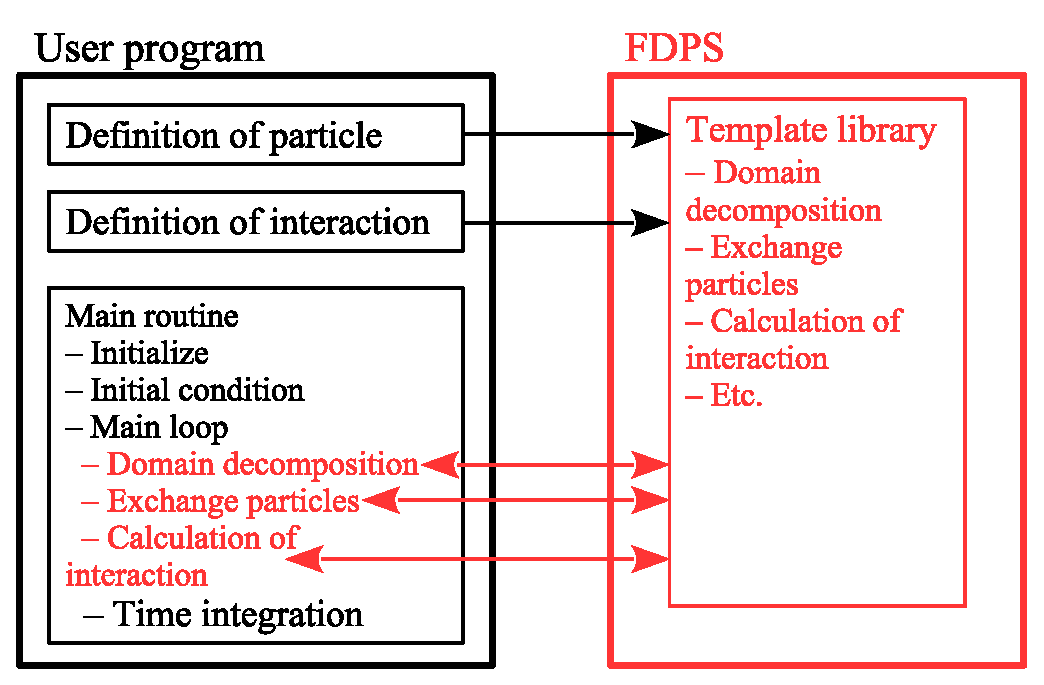
\includegraphics[width=8cm]{fig/concept.eps}
  \end{center}
  \caption{The basic concept of FDPS. The user program gives the
    definitions of particle and interaction to FDPS, and calls FDPS
    APIs.}
  \label{fig:concept}
\end{figure}

A user of FDPS can develop the simulation code in the following three
steps:
\begin{enumerate}
\item Define the data structure for $\myvec{u}_i$, as a class in C++
  language.
\item Define the function $\myvec{f}$. It should be a function object
  in C++ language\footnote{A function pointer of C language can be
    operable.}, which receives arrays of $i$-particles and
  $j$-particles, and calculates and accumulates $\myvec{f}$ on
  $i$-particles.
\item Write the user program using the data class and functions
  provided by FDPS. Currently, the user program should also be written
  in C++.
\end{enumerate}

Figure~\ref{fig:concept} illustrates how the user-defined code and
FDPS functions interact. The user program gives the definition of
particle and particle-particle interaction to FDPS at the compile
time. When executed, the user program first does the initialization
(the setup of MPI communication is done through a single call to an
FDPS initialization function), and the setup of the initial
condition. Then, the main integration loop is executed. In the main
loop, first the domain decomposition and exchange of particles are
performed, and then the calculation of interactions is
performed. These are all done through library calls to FDPS
functions. Finally, the time integration of particles using the
calculated interaction is performed.

In the above description, the interaction calculation is done once per
one iteration of the main loop. It is possible to use integration
schemes which requires multiple evaluations of interaction within a
single timestep, such as Runge-Kutta schemes. One can just call
interaction calculation API of FDPS, with $\myvec{u}_i$ containing
necessary intermediate values.

FDPS takes care of parallelization using MPI, and it can also use
OpenMP parallelization for internal operations and also for
interaction calculation. Thus, an FDPS user does not have to worry
about these issues. The efficient use of the cache memory and the SIMD
execution unit is not directly taken care by the FDPS libraries, but
handled through the interface to the user-defined interaction
calculation function. The interface is defined so that the interaction
calculation is done for multiple $j$-particles and multiple
$i$-particles. Thus, it performs a large amount of calculation, on a
small amount of data, since the calculation cost is the product of the
numbers of $i$- and $j$-particles, and data amount is sum of them.  In
order to make efficient use of the SIMD execution unit, the innermost
loop should be written in such a way that can be recognized as the
candidate of vectorization by the compiler used. The interface is
defined as taking AoS (array of structures) arguments.  Some compilers
for some architecture might not be able to generate the code to
utilize the SIMD unit for AoS data. In such a case, the user should
write the interaction function in which the AoS data is converted
internally to SoA (structure of arrays) data, and converted back to
the AoS form after the interaction is actually calculated.

\begin{figure}
  \begin{center}
    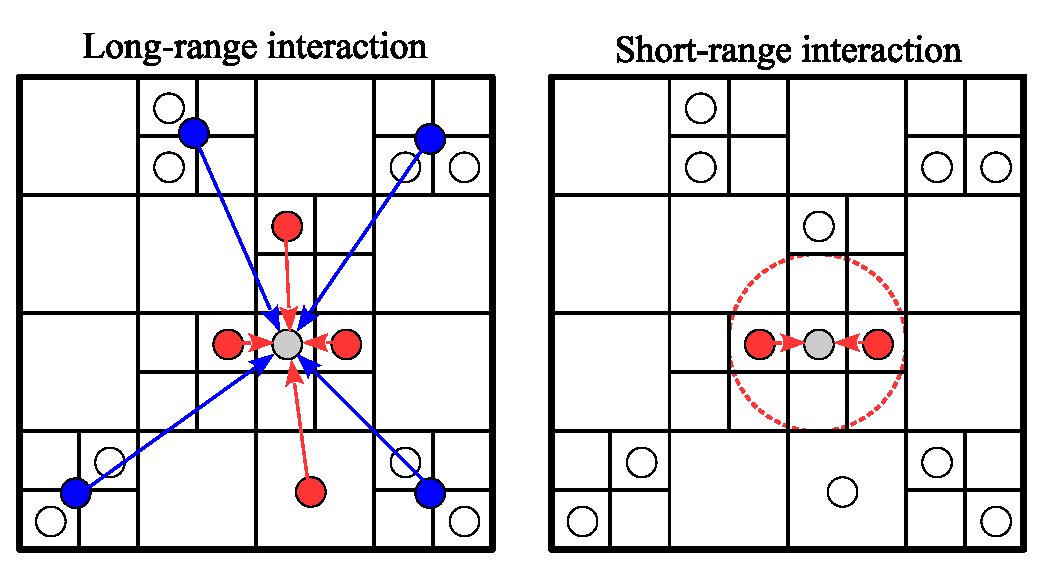
\includegraphics[width=8cm]{fig/force_type.eps}
  \end{center}
  \caption{Long-range interaction (left) and short-range interaction
    (right). Gray, red, and blue points are $i$-particle,
    $j$-particle, and superparticle, respectively.}
  \label{fig:forcetype}
\end{figure}

One might think that the definition of the system given in
equation~(\ref{eq:geq})  implies that  FDPS has to calculate $N^2$
interactions. If that were the case, FDPS would only be useful for
small problems. We implemented $O(N)$ and $O(N\log N)$ calculation
algorithms, for short-range and long-range interactions.

Within FDPS, the difference between long-range and short-range
interactions is slightly different from the physical one of infinite
and finite effective ranges. When we can and want to apply
multipole-like expansion to the contribution from distant particles,
we regard that interaction as long-range. The example of the
long-range interaction is gravity and Coulomb interaction in the open
boundary. When periodic boundary is used, they are usually evaluated
%using $\rm P^3M$ or PME method \cite{hockney1988computer}, in which
using $\mathrm{P^3M}$ or PME method \cite{hockney1988computer}, in
which the long-range part is evaluated using FFT, and only the
interaction with long-range cutoff is evaluated directly.  Even in
this case, we can still apply multipole interaction as used in TreePM
method \cite{1995ApJS...98..355X, 2000ApJS..128..561B,
  2002JApA...23..185B, 2004NewA....9..111D, springel:gadget2,
  2005PASJ...57..849Y, ishiyama:greem, ishiyama:gordonbell}, and in
this case the interaction is treated as long-range in FDPS.

For long-range interactions, FDPS uses standard Barnes-Hut tree
algorithm \cite{1986Natur.324..446B, 1990JCoPh..87..161B} parallelized
for distributed-memory machines and optimized for cache memory and
SIMD units \cite{ishiyama:greem, ishiyama:gordonbell}. For short-range
interactions, interaction list, or ``neighbor list'' for a group of
$i$ particles is constructed using a tree-based search, and that list
is used for the actual interaction calculation.
Figure~\ref{fig:forcetype} illustrates the long-range and short-range
interactions and how they are calculated in FDPS

For the long-range interaction, a multipole-like interaction is
used. Thus, equation~(\ref{eq:geq}) is modified to 
\begin{align}
  \frac{d\myvec{u}_i}{dt} = \myvec{g}\left( \sum_j^{N_{\mathrm{J},i}}
  \myvec{f}(\myvec{u}_i,\myvec{u}_j) + \sum_{j'}^{N_{\mathrm{S},i}}
  \myvec{f'}(\myvec{u}_i,\myvec{u'}_{j'}), \myvec{u}_i
  \right), \label{eq:geqL}
\end{align}
where $N_{\mathrm{J},i}$ and $N_{\mathrm{S},i}$ are, the number of
$j$-particles and superparticles for which we apply multipole-like
expansion, the vector $\myvec{u'}_{j'}$ is the physical quantity
vector of a superparticle, and the function $\myvec{f'}$ indicates the
interaction exerted on particle $i$ by the superparticle $j'$. In
simulations with a large number of particles $N$, $N_{\mathrm{J},i}$
and $N_{\mathrm{S},i}$ are many orders of magnitude smaller than $N$.
The user should also specify how superparticles are constructed from
ordinary particles, and also from superparticles in the lower level of
the tree. For $1/r$ potential, which is the typical usage of the
long-range interaction, FDPS provides the default way of construction
of superparticles up to the quadrupole moment.

In the case of the short-range interaction, the calculation of
contribution of distant particles is suppressed. Thus,
equation~(\ref{eq:geq}) is modified to
\begin{align}
  \frac{d\myvec{u}_i}{dt} = \myvec{g}\left(\sum_j^{N_{\mathrm{J},i}}
  \myvec{f}(\myvec{u}_i,\myvec{u}_j), \myvec{u}_i
  \right), \label{eq:geqS}
\end{align}
As in the case of the long-range force, $N_{\mathrm{J},i}$ is much
smaller than $N$, and usually independent of $N$.



% LocalWords:  FDPS subdomains subdomain MPI parallelization dt discretized API
% LocalWords:  APIs timestep Runge Kutta OpenMP SIMD vectorization AoS SoA PME
% LocalWords:  multipole FFT TreePM parallelized superparticles superparticle
% LocalWords:  quadrupole
